\section{Results}\label{results}

    \subsection{Roll decay model tests}\label{roll-decay-model-tests}

\subsubsection{0 knots}\label{knots}

Data from two roll decay model tests conducted at zero speed were
available
.
These tests where analyzed by fitting a cubic model
to the model test data. The two models were very similar in terms of
roll damping and stiffness (see fig.\ref{fig:mdl}), suggesting
good repeatability in the model tests as well as in the parameter
identification technique (PIT) used. The individual damping from each
oscillation obtained with the logarithmic decrement method are very
scattered, but this does not seem to influence the two models for the 0
speed case, which are very similiar.

    \subsubsection{15.5 knots}\label{knots}

Data from one roll decay model tests conducted at a ship speed
corresponding to 15.5 knots full scale ship speed was also available
(see fig.\ref{fig:mdl}). This model tests was analyzed in the
same way as the other tests. It was found that the damping was higher at
speed. The ship got a small yaw rate
 at the end of test, giving a small steady roll angle due to the
centrifugal force. Since this effect is not included in the matematical
model used, the steady roll angle was instead removed by removing the
linear trend in the roll angle signal.

    

    \begin{figure}[H]
        \begin{center}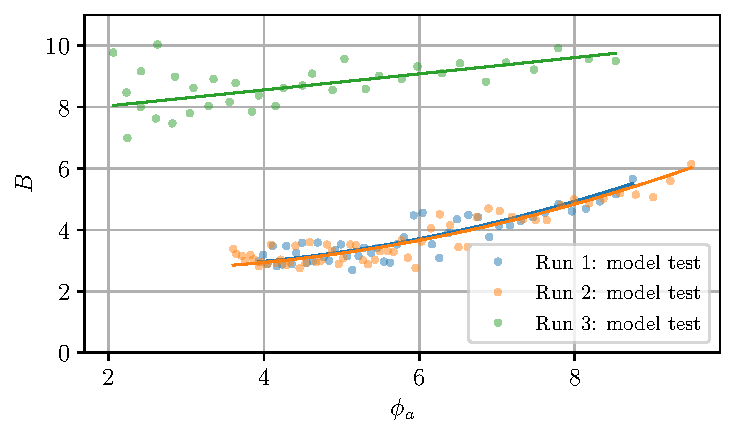
\includegraphics[width = 0.5\textwidth]{figures/mdl.pdf}\end{center}
        \vspace{-1cm}
        \caption{Model test roll damping}
        \label{fig:mdl}
    \end{figure}
    
    \subsection{Ikeda's method}\label{ikedas-method}

    The $C_r$ was predicted with Ikeda's method and the alternative
decision tree model for the KVLCC2 with section data according to
tab.\ref{tab:kvlcc2_section_table}. A comparison is shown in the
figure below, where it can be seen that the Ikeda implementation
predicts much higher $C_r$ between station 8 and 14, where the bilge
radius is also very small.

    \begin{figure}[H]
        \begin{center}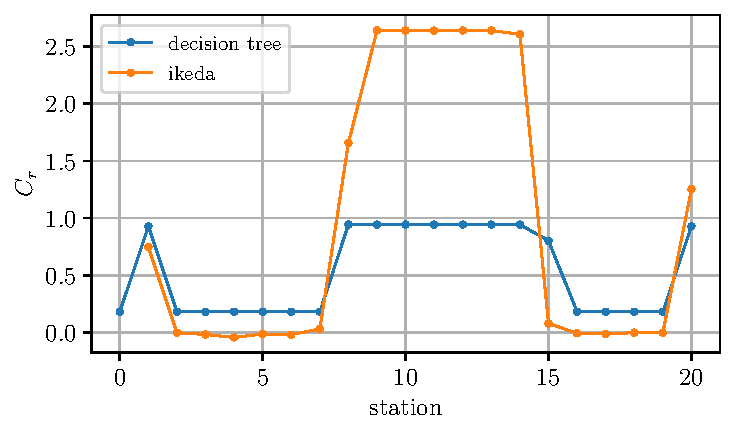
\includegraphics[width = 0.5\textwidth]{figures/kvlcc2_eddy.pdf}\end{center}
        \vspace{-1cm}
        \caption{KVLCC2 eddy damping coefficient along the hull}
        \label{fig:kvlcc2_eddy}
    \end{figure}
    
    When looking at predictions in fig.\ref{fig:ikeda} for KVLCC2 at
0 speed made with regular Ikeda's method (left), it was found that the
eddy damping $B_E$ was too high compared to the model test results.
Even though the rest of the components would also be overpredicted, the
$B_E$ would still be too large. The eddy damping calculated with
$C_r$ predicted with the descision tree gave much better agreement.

    

    \begin{figure}[H]
        \begin{center}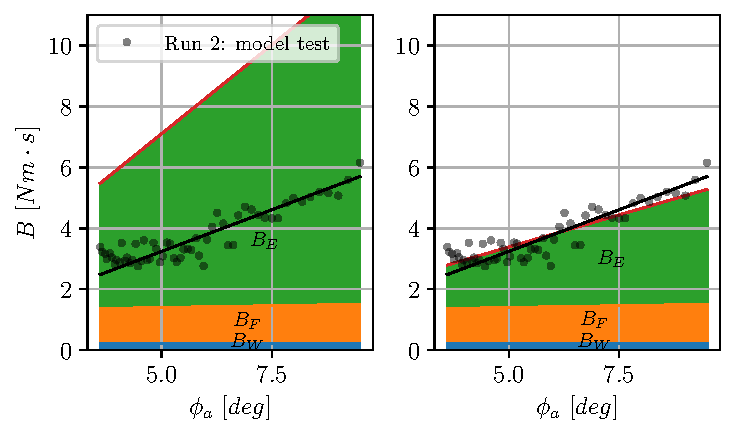
\includegraphics[width = 0.5\textwidth]{figures/ikeda.pdf}\end{center}
        \vspace{-1cm}
        \caption{Roll damping components calculated with the two Ikeda implementations.}
        \label{fig:ikeda}
    \end{figure}
    
    \subsection{FNPF}\label{fnpf}

Simulations of roll decay tests were conducted with FNPF without viscous
damping. Wave damping obtained from these tests are shown in
fig.\ref{fig:fnpf}. It looks like this damping term does not
change much with the amplitude making it reasonably linear, which is in
line with Ikeda's original assumption for the derivation of eddy damping
\cite{7505983/4AFVVGNT}.

    

    \begin{figure}[H]
        \begin{center}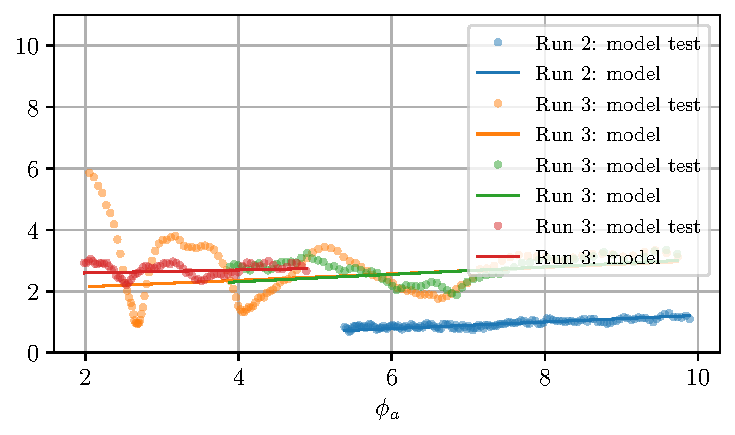
\includegraphics[width = 0.5\textwidth]{figures/fnpf.pdf}\end{center}
        \vspace{-1cm}
        \caption{Wave damping obtained from FNPF}
        \label{fig:fnpf}
    \end{figure}
    
    \subsection{Roll motion prediction with hybrid
method}\label{roll-motion-prediction-with-hybrid-method}
Replacing the wave damping $B_W$, for the zero speed case above, with values obtained with FNPF is shown below. 
    \begin{figure}[H]
        \begin{center}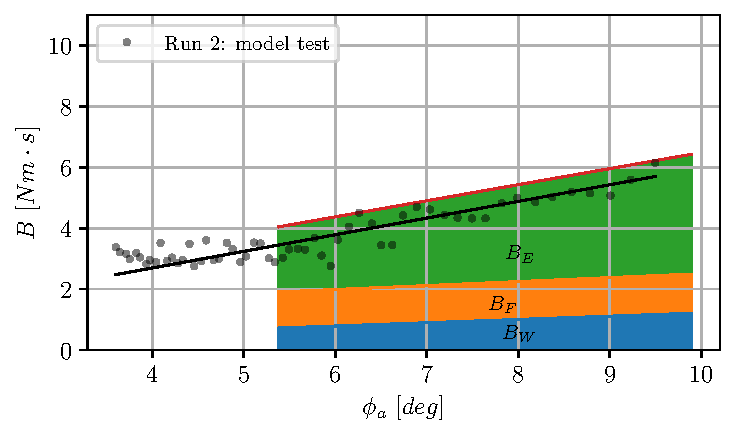
\includegraphics[width = 0.5\textwidth]{figures/hybrid_0.pdf}\end{center}
        \vspace{-1cm}
        \caption{Roll damping from hybrid method (0 kn)}
        \label{fig:hybrid_0}
    \end{figure}
    
    Results from the roll decay model test and corresponding simulations
with hybrid method and FNPF method is shown in the figure below. It can
be seen that the injection of semi empirical viscous damping in the
hybrid method has given a significant improvement to the FNPF roll
motion prediction.

    \begin{figure}[H]
        \begin{center}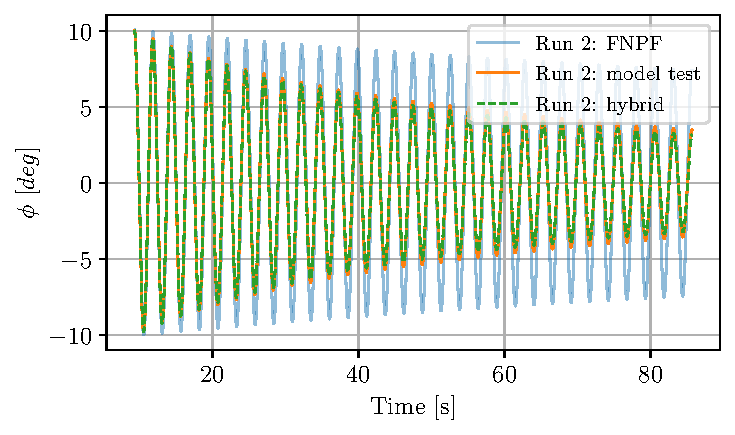
\includegraphics[width = 0.5\textwidth]{figures/hybrid_0_time.pdf}\end{center}
        \vspace{-1cm}
        \caption{Roll decay (0 kn)}
        \label{fig:hybrid_0_time}
    \end{figure}
    
    The total damping from the hybrid method is similar to the model test
results for the zero speed case. For the in speed case the agreement is
however even better:

    \begin{figure}[H]
        \begin{center}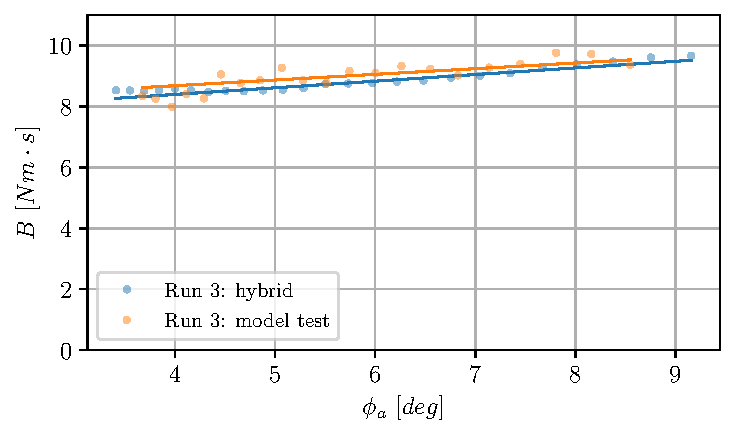
\includegraphics[width = 0.5\textwidth]{figures/hybrid_speed_amplitudes.pdf}\end{center}
        \vspace{-1cm}
        \caption{Roll damping from hybrid method (15.5 kn)}
        \label{fig:hybrid_speed_amplitudes}
    \end{figure}
    
    Results from roll decay tests are shown for the in speed case below.

    \begin{figure}[H]
        \begin{center}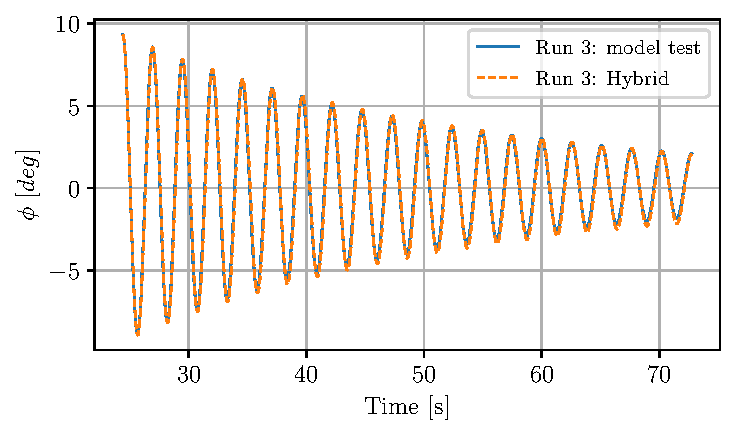
\includegraphics[width = 0.5\textwidth]{figures/hybrid_speed_time.pdf}\end{center}
        \vspace{-1cm}
        \caption{Roll decay (15.5 kn)}
        \label{fig:hybrid_speed_time}
    \end{figure}
    
    The coefficients obtained from model tests, FNPF and hybrid method are
summarized in model scale units in the table below. The equivalent
linearized damping for 5 degrees roll angle amplitude $B_{e5}$ has
also been added to this table, for comparison. It can be seen that the
hybrid method overpredicts the damping at 0 knots and underpredicts the
damping for the higher speed at this amplitude.
 
            
    
    
\begin{table}[H]
\scriptsize
\center
\caption{Roll damping coefficients for model scale KVLCC2}
\label{tab:results}
\begin{tabular}{llllll}
\toprule\addlinespace
$F_n$ & method & $B_1$ & $B_2$ & $B_3$ & $B_{e5}$\\ 
\midrule$[-]$ &  & $[Nm \cdot s]$ & $[Nm \cdot s^2]$ & $[Nm \cdot s^3]$ & $[Nm \cdot s]$\\ 
0.0 & model test & 2.9604 & -6.5205 & 43.7754 & 3.2864\\ 
0.0 & model test & 2.8797 & -5.8742 & 41.5037 & 3.2447\\ 
0.0 & Hybrid & 1.3711 & 13.4769 & 0.0 & 3.828\\ 
0.1423 & model test & 7.5233 & 7.0281 & 0.3898 & 8.8214\\ 
0.1423 & Hybrid & 7.5216 & 6.0148 & 0.0 & 8.6095\\ 

\bottomrule
\end{tabular}
\end{table}

    

    